% This is samplepaper.tex, a sample chapter demonstrating the
% LLNCS macro package for Springer Computer Science proceedings;
% Version 2.20 of 2017/10/04
%
\documentclass[runningheads]{llncs}
%
\usepackage[utf8]{inputenc}
\usepackage{graphicx}
\usepackage[british]{babel}
\usepackage{amsmath}
\usepackage[linesnumbered]{algorithm2e}
\usepackage{algorithmic}


%\usepackage[backend=biber]{biblatex}
%\usepackage[backend=biber,style=splncs04]{biblatex}  %backend=biber is 'better'  

% Used for displaying a sample figure. If possible, figure files should
% be included in EPS format.
%
% If you use the hyperref package, please uncomment the following line
% to display URLs in blue roman font according to Springer's eBook style:
% \renewcommand\UrlFont{\color{blue}\rmfamily}

% ---- Bibliography ----
%
% BibTeX users should specify bibliography style 'splncs04'.
% References will then be sorted and formatted in the correct style.
%
\DeclareMathOperator{\sgn}{sgn}


\newcommand{\xn}{\ensuremath{\mathbf{x_0}}}
\newcommand{\xb}{\ensuremath{\mathbf{x}}}
\newcommand{\rb}{\ensuremath{\mathbf{r}}}
\newcommand{\vb}{\ensuremath{\mathbf{v}}}
\newcommand{\kf}{\ensuremath{k_{\!f}}}
\newcommand{\kg}{\ensuremath{k_{\!g}}}
\bibliographystyle{splncs04}
\begin{document}
%
\title{Combining Universal Adversarial Perturbations on two Networks}%\thanks{Supported by organization x.}
%
\titlerunning{Combining Universal Adversarial Perturbations}
% If the paper title is too long for the running head, you can set
% an abbreviated paper title here
%
\author{Maurus K\"uhne\inst{1}\orcidID{0000-0002-4205-3552} \and
Beat Tödtli\inst{2}\orcidID{0000-0003-3674-2340}} %\and
%Third Author\inst{3}\orcidID{2222--3333-4444-5555}}
%
\authorrunning{M. Kühne and B.Tödtli}
% First names are abbreviated in the running head.
% If there are more than two authors, 'et al.' is used.
%
\institute{Fernfachhochschule Schweiz\\
\url{ffhs.ch}\and
Institut für Informations- und Prozessmanagement, FHS St.Gallen, \\
\email{beat.toedtli@ost.ch}\\
\url{fhsg.ch} 
}
%
\maketitle              % typeset the header of the contribution
%
\begin{abstract}
Universal adversarial perturbations (UAPs) are small perturbations imposed on images that are able to fool a single convolutional neural network image classifier. They have been shown to generalize well to other neural networks. Here, we report on our reproduction effort of the results given in~\cite{moosavi-dezfooli_universal_2017} and study two methods to construct UAPs for several neural networks. While the results are not strong enough to make general conclusions, they suggest that UAPs indeed profit from being constructed on several neural networks. Also, we show that a linear interpolation between two UAPs does not produce a viable UAP on both networks.
%\cite{yu_generating_2018}
\keywords{Adversarial Training\and Universal Adversarial Perturbation}
\end{abstract}
%
%
%

\section{Introduction}
The discovery of Szegedy et al.~\cite{Szegedy_2014} that several machine learning models including deep neural networks are vulnerable to \emph{adversarial attacks} was seminal for a new subfield of studying deep learning. Probably the most intriguing, but also unsettling result was that adversarial examples can be made quite imperceptible to the human eye, while still fooling a convolutional neural network to misclassify the image~\cite{goodfellow_2014}. Subsequent work has developed various algorithms in a variety of white-box, gray-box and black-box attack scenarios as well as defensive strategies such as adversarial training~\cite{REN2020346}. Moosavi-Dezfooli et al. have demonstrated that \emph{universal} perturbations exist, i.e. that a single set of of pixel modifications can be found that fools a network on a large fraction of the training data set~\cite{moosavidezfooli_universal_2017}. Moreover, universal adversarial perturbations (UAPs) also fool other convolutional networks, albeit to a lesser but still very significant degree~\cite{moosavidezfooli_universal_2017}. 

These results suggest that neural networks partly share a common structure that can be exploited by universal adversarial perturbations (UAPs), while yet other aspects are different. Much remains to be understood about the shape of the decision surfaces in neural networks and how they depend on the architecture of the neural network. In this context, we ask how the transferability of UAPs to new convolutional neural networks can be improved by combining two neural networks in the adversarial perturbation generation algorithm. By combining two neural networks in the generation process of adversarial examples, one might expect to see an increase in the transferability of an adversarial perturbation to other networks. Ultimately, we hope this approach will lead to identifying a general property resulting in convolutional neural networks being susceptible to adversarial attacks.

Given the practical potential and relevance of Deep Learning and the above potential security threats, finding a robust resolution is important and urgent. However, research into the topic is hampered by the \emph{reproducibility crisis} in machine learning~\cite{raff2020quantifying}. A lot of research results, including on adversarial attacks, remain poorly documented in publications. While the methods described may be general enough to be useful for many similar applications, 
the published results are often difficult to reproduce due to undocumented values for hyperparameters, software library versions etc.~\cite{Gundersen2018StateOT}. % {\bf ev. https://arxiv.org/vc/arxiv/papers/1909/1909.03032v1.pdf zitieren?}
Also, only in rare cases is it clear how well the published results generalize beyond the very specific data set that was used but not provided to produce the published results. While not being able to reproduce the generation of adversarial examples may seem beneficial at first sight, it is clear that a thorough resolution of such security issues requires a well-stated problem, including readily available state-of-the-art algorithms for the production of adversarial examples. They form the basis of being able to test deep learning systems against such attacks. 

The authors of~\cite{moosavidezfooli_universal_2017,moosavi-dezfooli_deepfool_2016} show good generalization results for UAPs generated with their procedure \emph{DeepFool}~\cite{moosavi-dezfooli_deepfool_2016} across different deep learning architectures. We report on our reproduction effort, provide our code and investigate whether modifications of their UAP algorithm are able to improve the generalization capability of UAPs by using modifications of the UAP generation algorithm that take into account several networks at the same time. Specifically, we ask whether incorporating information from a second neural network architecture improves the fooling rate of UAPs on a third neural network. We investigate three {\bf CHECK!} combination procedures and compare them with the original adversarial attack procedure.

This paper is organized as follows. After an introduction to DeepFool and the construction of UAPs, we describe our reproduction effort of the original work of Moozavi-Dezfooli et al.~\cite{moosavidezfooli_universal_2017}. We then present several modifications of their UAP generation algorithm to construct UAPs that are optimized on two networks. We present our results that compare these variants to the original UAP generation algorithm of Moozavi-Dezfooli et al. We conclude with a discussion of these results.

\section{Methods}
\subsection{General Setting}
Given a classifier \(\hat{k}(x)=\sgn\left(f(x)\right)\) that is based on the sign of a classification function \(f:\mathbf{R}^n\rightarrow\mathbf{R}\), adversarial attacks seek a perturbation \(\vb\) such that \[\hat{k}(\xb+\vb)=\sgn\left(f(\xb+\vb)\right)\neq \sgn\left(f(\xb)\right)=\hat{k}(\xb).\] 


\subsection{DeepFool}
In DeepFool, the perturbation \(\mathbf{v}\) for an image \(\xn\) is defined to be the shortest vector (using the \(L_2\)-norm \(\left\|.\right\|\)) such that \(\xn+\mathbf{v}\) lies on a decision boundary. 
If $f(\xb)$ is a linear function $f(\xb)=\mathbf{w} \xb+\mathbf{b}$, then \(\mathbf{v}\) can be shown to be \(\mathbf{v}=-\frac{f(\xn)}{\left\|\mathbf{w}\right\|_2^2}\mathbf{w}\). As \(f\) is nonlinear in general, the Taylor approximation \(f(\xb)=f(\xn)+\left(\nabla f(\mathbf{x})\right)^T\mathbf{v}\) is used to iteratively reach the decision boundary. 
In the multi-class setting considered here, there is an additional step of identifying the closest decision boundary. 
% where \(\xi\) is a hyperparameter.{\bf stimmt das??} For Details, see~\cite{DeepFool-Moosavi-Dezfooli15}. \\


\subsection{Multi-Classifier-Universal adversarial Perturbations with DeepFool}\label{sec:MultUAP}

Perturbations for each image in a dataset \(X\) (such as those generated using DeepFool) can be combined to form universal adversarial perturbations for a single network~\cite{moosavidezfooli_universal_2017}. The procedure is given in Alg.~\ref{alg:3}. Essentially, DeepFool perturbations of images that are not yet misclassified are added to obtain a universal perturbation. 
Whenever the norm of the perturbation becomes large, a rescaling is applied. The perturbation is scaled back to satisfy a norm bound given by \(\left\|\mathbf{v}\right\|_2\leq\xi\). For a small value of \(\xi\), this ensures that the perturbation remains largely invisible. Hence images added later in the UAP-Generation may have a larger impact on the perturbation $\xb$ than the previous ones. For details, see~\cite{moosavidezfooli_universal_2017}. 

Intriguingly, although the directions to the class boundaries vary for different training images, the resulting average over all image perturbations works well according to~\cite{moosavidezfooli_universal_2017}, even for other convolutional neural networks whose class boundaries might be expected to look rather different. 

In the following subsections, we detail two approaches at generating UAPs for several classifiers.

\subsubsection{Alternated generation of perturbations}
As UAPs are constructed by adding up the perturbations generated using DeepFool, there is a natural way to combine perturbations generated by the two networks: We add up the contributions from two networks alternatingly, hoping that the selection of images that are not yet fooled is sufficient to guide the perturbation generation process. The precise procedure used here is given in Alg.~\ref{alg:3}. The procedure naturally generalizes to multiple neural networks. 

Variants of Alg.~\ref{alg:3} exist that sample the images differently. One might for example generate perturbations for one image from both neural networks, instead of alternatingly using a single network on an image sample. We note that adding up the perturbations is not a commutative operation, since projections take place once the size (norm) of the perturbation becomes too large. 
{\bf CHECK In our experience, these variations do not significantly change the fooling rates}.
 
\subsubsection{Interpolation between UAPs on individual networks}
A simple yet instructive alternative to the above rather involved perturbation construction is given by a simple weighted average of the perturbation vectors generated on the individual networks. If we restrict our attention to the combination of two neural networks for now, then the weighted averages of the perturbations lie on a line in the high-dimensional vector space of images. In the following, we specifically investigate whether any perturbation lying on this line improves on the fooling capability of the two endpoints with respect to a third network.
More formally, given UAPs \(\mathbf{v}_f\) and \(\mathbf{v}_g\) of two neural networks $f$ and $g$, we consider \begin{equation}\label{eq:interp}
\mathbf{v}_{fg}\left(\lambda\right)=\lambda\,\mathbf{v}_f+\left(1-\lambda\right)\mathbf{v}_g
\end{equation}	
for values \(\lambda\in\left[0,1\right]\). We seek the value of $\lambda$ that maximizes the average fooling rate over $f$, $g$ and a third network, given the current training data set.


\subsubsection{Outlook to other approaches}
We have also investigated other, more involved approaches that led to unsatisfactory results. In particular, we were interested in constructing a multi-class DeepFool procedure that uses the gradients of two networks towards the next class boundary to compute a perturbation of a single image. One might try to find perturbations towards class boundaries that are aligned as much as possible, but where the class boundaries correspond to different classes in different networks. As of now, these attempts have not provided efficient UAPs for multiple networks.

%{\bf alter Satz, ev. nützlcihe idee?} We seek the perturbation which points in the averaged direction of the two single-network perturbations, with a strength proportional to the sums of the of the (absolute)  changes in activation when compared to the unperturbed image. {\bf seehr shaky!!! Besser motivieren!!}
\begin{figure}
\begin{algorithm}[H]\label{alg:3}

\SetAlgoLined
{\bf Input}:Data set \(X\), a set of classifiers \(K\), desired norm \(\left\|.\right\|_p\) of
the perturbation \(\xi\)\;
{\bf Output}: Universal perturbation vector \(\vb\)\;
Initialize \(\vb \gets 0\)\;%, epoch\gets 1\;\;

\While{\textup {Average fooling rate is too low}}{
\ForEach{\(\mathrm{image~}\xb\in X\)  }{ 
\ForEach{\(\hat{k}\in K\)  }{ 
	%\(\Delta \mathbf{r}_k\gets\mathrm{UAP} (k)\)\;
	\If{ \(\hat{k}(\xb)=\hat{k}(\xb+\vb)\)}{
	%\(\Delta \rb\gets \underset{r}{\arg \min}\left\|r\right\|_2~\mathrm{s.t.}~\hat{k}(\mathbf{x}+\rb+\Delta\rb)\neq\hat{k}(\mathbf{x})\)\;
		\(\Delta \vb\gets\mathrm{DeepFool} (\xb+\vb,\hat{k})\)\;
	\(\vb\gets \vb+\Delta \vb\)\;  
	\(\vb\gets \sqrt{\xi}\vb/\left\|\vb\right\|_p\)
}  }
} 
 }
\Return \vb
 \caption{Computation of universal adversarial perturbations for multiple neural networks. }
\end{algorithm}
\end{figure}

\section{Results}
In this section we first discuss our attempt at the reproduction of the results in~\cite{moosavidezfooli_universal_2017} regarding the transferability of UAPs accross neural network architectures. We then provide the results of our attempts at constructing UAPs based on two neural network architectures at the same time.

\subsection{Reproduction of the Original Results on Universal Adversarial Perturbations}
Dezfooli et al. tested the DeepFool and Universal Adversarial Perturbations algorithms on 5 different neural networks~\cite{moosavidezfooli_universal_2017}. We choose networks similar to the ones used in~\cite{moosavidezfooli_universal_2017} that have publicly available pretrained weights. We compare the achieved fooling rates with those given in the original paper. Separate experiments have been performed by training individual UAPs on each of the networks, and subsequently measuring the fooling rates on all available networks. All perturbations were generated using the same random subset of 10'000 images of the ImageNet training set~\cite{imagenet_cvpr09}, and the fooling rates were measured on the ImageNet validation set (containing 50'000 images).

\begin{figure}[h]\label{fig:UAPs}
	\centering
		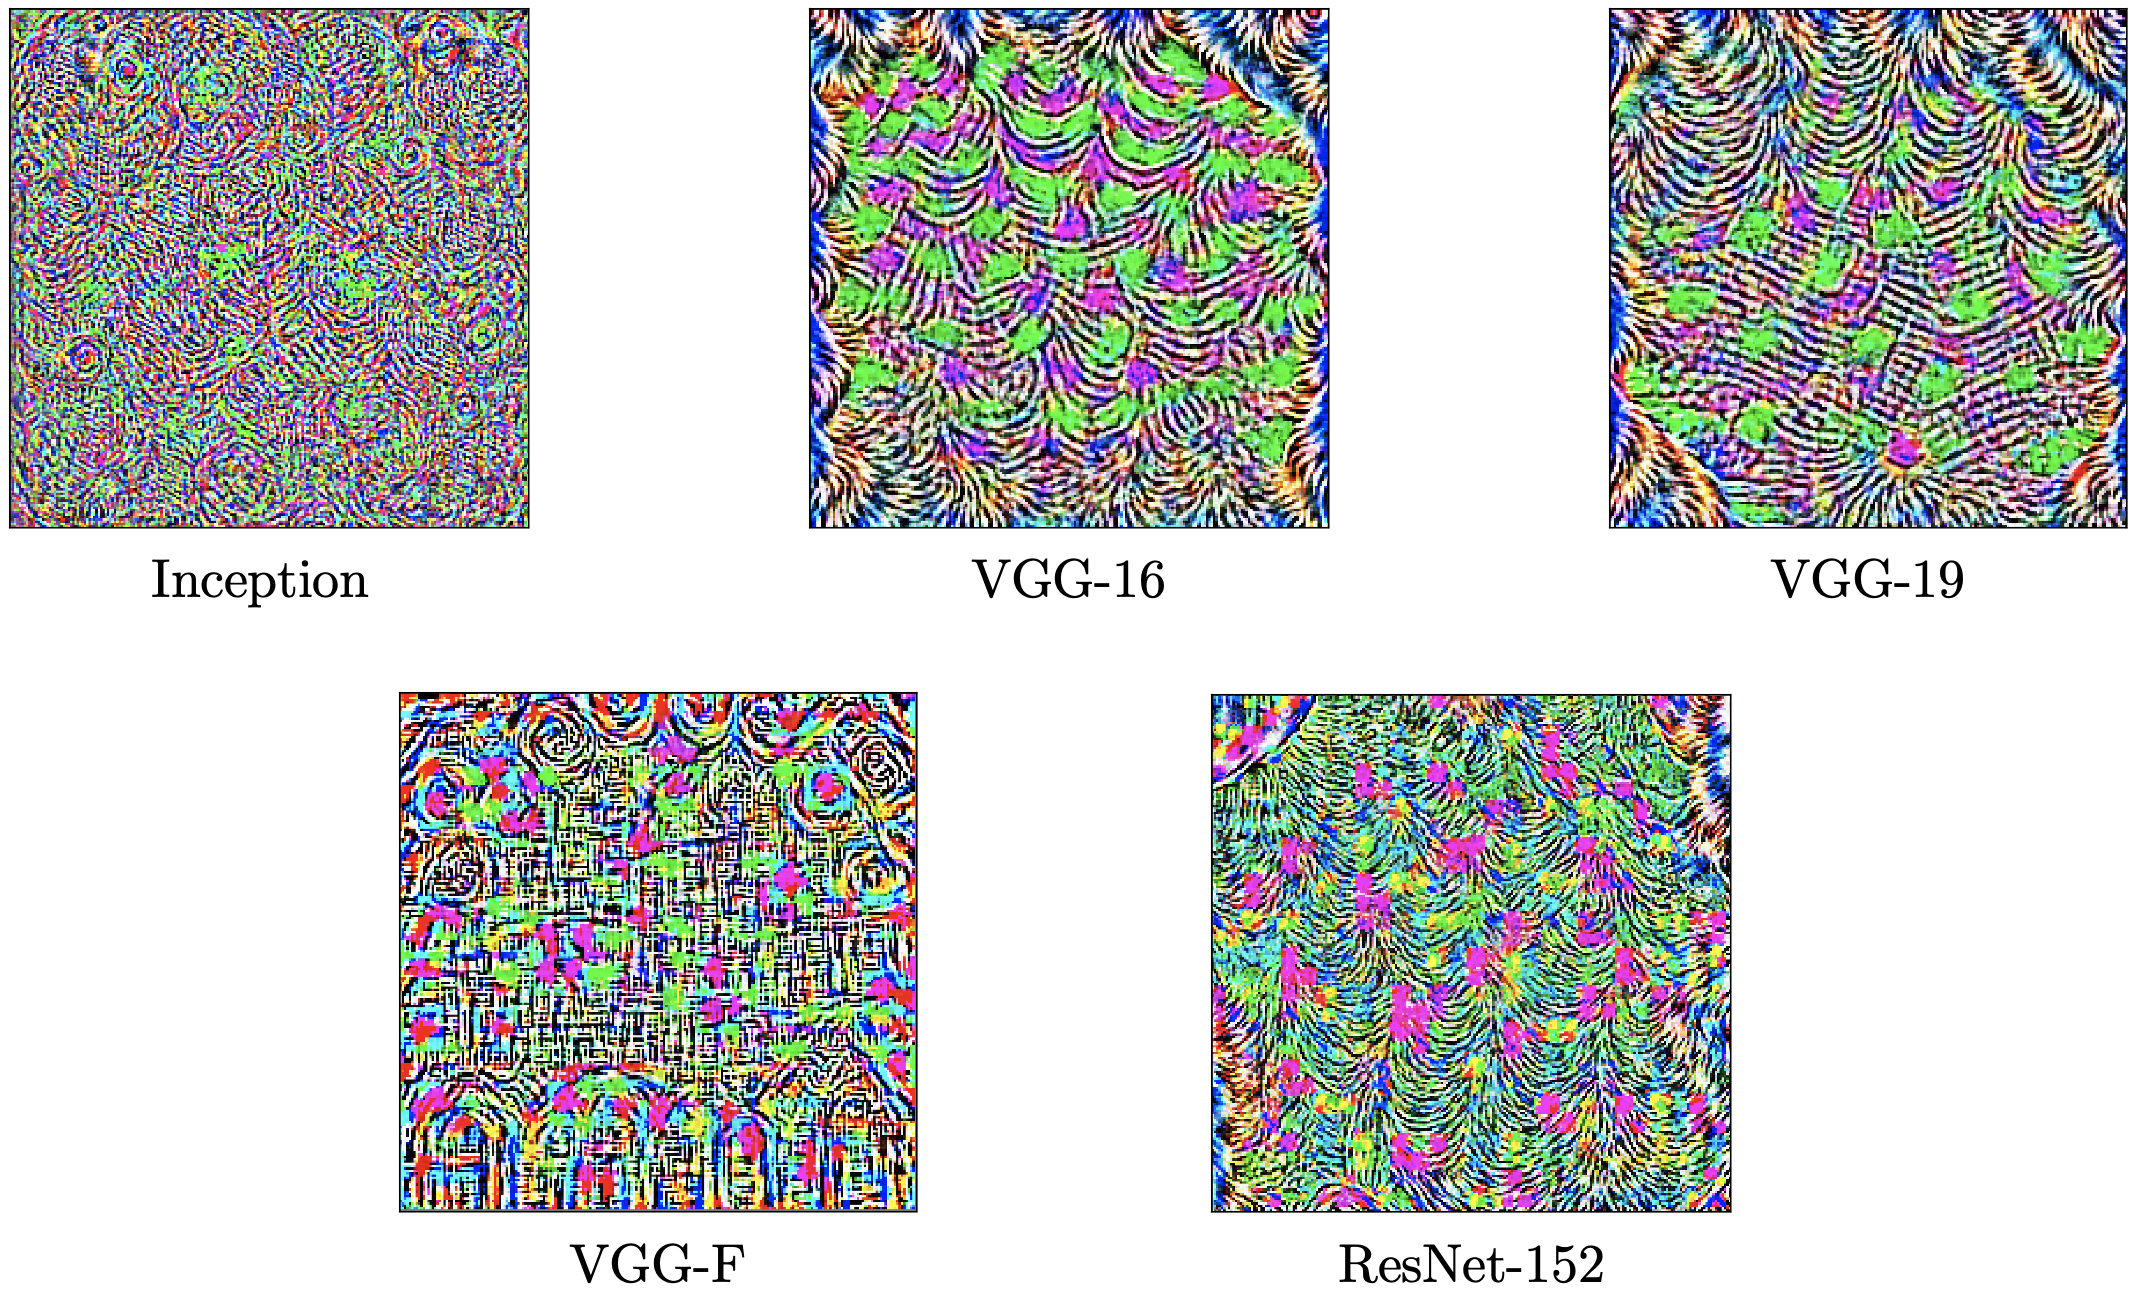
\includegraphics[width=1.0\textwidth]{images/own_perturbations.png}
	\label{fig_stoerwerte}
	\caption{Visualisation of the generated perturbations. To visualise the perturbations we shifted them by $+\xi$ and extended them to the entire color space with a scalar multiplication.}
\end{figure}

Figure~\ref{fig:UAPs} shows the perturbations generated. In their general structure and appearance, they are similar to the ones reported in~\cite{moosavidezfooli_universal_2017}. As the structures seen in Fig.~\ref{fig:UAPs} are quite particular, we believe that this indicates that deviations from the original results reported below probably stem from configuration details rather than a fundamental reproduction mistake.

\begin{table}[htbp]
\centering
\caption{Fooling rates for the ImageNet validation set.}
\begin{tabular}{|l|l|l|l|l|l|}
\hline

			& VGG-F		&	Inception	&	VGG-16		&	VGG-19		&	ResNet-152	\\ \hline
VGG-F		& $90\%$	&	$56\%$		&	$32\%$		&	$32\%$		& 	$24\%$		\\
Inception	& $42\%$	&	$82\%$		&	$16\%$		&	$16\%$		& 	$16\%$	\\
VGG-16		& $46\%$	&	$60\%$		&	$59\%$		&	$52\%$		& 	$38\%$	\\
VGG-19		& $45\%$	&	$58\%$		&	$51\%$		&	$54\%$		& 	$33\%$	\\
ResNet-152	& $42\%$	&	$55\%$		&	$31\%$		&	$33\%$		& 	$73\%$	\\
\hline 
\end{tabular}
\label{tbl_stoerraten_reprod_kreuz_linf}
\end{table}

Table~\ref{tbl_stoerraten_reprod_kreuz_linf} shows the achieved fooling rates for the tested models and should be compared with Table 2 of  Moosavi-Dezfooli et al.~\cite{moosavidezfooli_universal_2017}. The first column indicates the network used to generate the UAP, while the first row gives the network on which the fooling rate is measured. The main diagonal therefore contains the self-fooling rates, i.e. the fooling rates achieved using the same model for generating the perturbation and measuring the fooling rate. 

In reproducing these numbers, several insufficiently documented design choices had to be researched. For example, the original results are not stated for a given epoch, but using a stopping condition on the error rate. Values reported here are for epoch 20, at which point the mean value over the last 5 epochs typically varies by less than 0.005. Parameter values taken from and in the notation of~\cite{DeepFool-Moosavi-Dezfooli15} are \(p=\infty\) and \(\xi=10\). We used a maximum of 10 DeepFool update iterations. The overshoot parameter \(\eta=0.02\) was again taken from~\cite{DeepFool-Moosavi-Dezfooli15}. 
%\footnote{Called $\text{num_classes}$ in the code given in 
%https://github.com/LTS4/universal.
%}
An important parameter is the number of class boundaries, called num\_classes\footnote{As given in the code at https://github.com/LTS4/}. It gives the number of class boundaries in whose direction a perturbation is searched for. Computation time is highly sensitive to this parameter, and checking all 1000 training boundaries of ImageNet was infeasible. Higher values generally improve the fooling performance, though exceptions are observed. 
Other minor parameters such as random initialisation values for the train-test split, etc. were taken from their provided code. We have tried to optimize these parameters using grid searches, but the available computing resources have limited these efforts. 

\subsection{Evaluation of Attempts to Construct Universal Adversarial Perturbations for Multiple Neural Networks}
In this section we present our results for constructing UAPs that make use of two neural networks. We discuss results for the two approaches presented in Sec.~\ref{sec:MultUAP}, the alternated generation of perturbations and the linear interpolation between UAP on individual networks.
%\subsubsection{Alternated generation of perturbations} WAS IST DAMIT?

The alternated generation of perturbations proceeded as given in Alg.~\ref{alg:3} and has been applied to the set of classifiers \(K=\left\{\text{Inception},\text{VGG-16}\right\}\). The fooling rates are reported for these two networks and for ResNet-152. Table~\ref{tab:vergleich_comb} has two sections. In the upper section, the network listed in the first column is used to generate the perturbation. The columns give the fooling rates on the network given in the column title as well as their average as our measure for the generalizability of the UAPs. We include the original network in this average. 

The second section reports results by applying the alternated generation of UAPs and the interpolation method given in Eq.~(\ref{eq:interp}) using the value $\lambda=0.05$. 

The alternated generation of a UAP on both networks (Alg.\ref{alg:3}) generated a perturbation that achieved slightly higher fooling rates on VGG-16 and ResNet-152 than a perturbation generated directly on VGG-16 (with an absolute increase of 2.1 and 3.2 percentage points, respectively). For Inception, the perturbation achieved a fooling rate of 67.4\%. This is 14.6\% below the measured self fooling rate of Inception (81.9\%), but 7.4\% higher than the fooling rate achieved with a VGG-16 model. 


Linear interpolation between the UAPs of VGG-16 and Inception V1 resulted in a best value of \(\lambda=0.05\) (see Eq.~(\ref{eq:interp})). Using this configuration, the fooling rates remained essentially unchanged compared to the UAP generated on VGG-16 only.
The value \(\lambda=0.05\) results in a perturbation that is similar to the VGG-16 perturbation as the VGG-16 perturbation is weighted with \(1-\lambda=0.95\), while the Inception perturbation contributes only with a weight of 5\%. Choosing \(\lambda\in\left[0.1,0.15,\ldots,0.4\right]\) resulted in perturbations with lower fooling rates for both models with respect to the rates achieved by separately training UAPs on the two networks. For \(\lambda \in\left[0.4,1.0\right]\), the fooling rates for Inception improved again, but did not exceed the fooling rates of a UAP generated on Inception itself. The fooling rates on VGG-16 continued to deteriorate, stabilizing at a low fooling rate of \~15\% after \(\lambda\geq 0.65\) {\bf Maurus, prüfen...}. 

{\bf Todo: Insgesamt besser!}

\begin{table}
\centering

\begin{tabular}{|l|l|l|l|l|l|}
\hline
											&	Inception	V1&	VGG-16		&	ResNet-152	& Average	\\ \hline
Inception V1 UAP							&	\(81.9\%\)		&	\(15.9\%\)	&	{\bf WF!}\(15.6\%\)	&37.8\%	\\
VGG-16 UAP								&	\(60.0\%\)		&	\(58.7\%\)	&	\(38.0\%\)	&52.2\%	\\
ResNet-152 UAP &	\(54.6\%\)		&	\(31.4\%\)	&	\(73.4\%\)&53.1\%		\\ \hline
linear interpolation (\(\lambda=0.05\))	&	\(59.9\%\){\bf WF?}		&	\(58.7\%\)	&	\(38.0\%\)	&\%\\
alternated generation of UAPs&	\(67.3\%\)		&	\(60.6\%\)	&	\(41.2\%\)		&56.4\%\\
alternated generation of UAPs (Variante 2)&	\(63.3\%\)		&	\(55.0\%\)	&	\(36.3\%\)	& \(51.5\%\)	\\

%Finetuning									&	$59.9\%$		&	$57.9\%$	&	$38.6\%$		\\
%modifiziertes DeepFool						&	$43.6\%$		&	$18.4\%$	&	$14.1\%$		\\
\hline 
\end{tabular}

\caption{Comparison of the fooling rates by UAPs trained on individual networks (upper three rows) and of the alternated generation  (Alg.~\ref{alg:3}) and linear interpolation (Eq.~(\ref{eq:interp})) procedures. Results are reported on the validation set, using the $l_\infty$-norm, $\xi=10$ and 20 UAP iterations.}\label{tab:vergleich_comb}
\end{table}


\section{Discussion}
\subsection{Reproduction of the Original Results on Universal Adversarial Perturbations}
For most models the fooling rates reported in the original paper could not be achieved. For VGG-F, VGG-16, VGG-19 and ResNet-152 our  self-fooling rates were between 4.1 and 23.5 absolute percentage points lower. For Inception we achieved a self-fooling rate 3 absolute percentage points higher than the one reported in the original paper. Clearly, this is not satisfactory and further research is needed to state the precise conditions under which a reliable reproduction of the reported fooling rates is possible. As a step in this direction we provide our code.\footnote{https://github.com/mauruskuehne/lwda-paper}

The non-diagonal values in Tab.~\ref{tbl_stoerraten_reprod_kreuz_linf} are large but typically significantly smaller than the diagonal values. They show a degree of transferability of UAPs generated with DeepFool to other models. Therefore, despite the reproducibility problems, these results broadly confirm that UAPs generated with DeepFool generalize to other network architectures. Nevertheless, it is clear that some aspects of UAPs are specific to a given neural network architecture. We discuss our results on finding a way to improve the non-diagonal elements (potentially at the cost of the diagonal ones) in the next section.
Interestingly, we achieved lower fooling rates than Moozavi-Dezfooli et.al, except for the Inception network, for which we achieve 3-8 absolute percentage points higher fooling rates. This may indicate that the Inception network is more susceptible to these perturbations. Another possibility are the chosen hyperparameter values for DeepFool and UAP, which may be particularly well suited or optimized for this model. This in turn would explain the lower fooling rates achieved on other models.

\subsubsection{Alternated generation of perturbations and linear Interpolation between UAP on individual networks}
As the results in Tab.~\ref{tab:vergleich_comb} clearly show, a linear interpolation between two UAPs does not give good results. One obvious candidate interpretation is that since neural networks are highly non-linear functions, there is no reason to assume that combining their UAPs as a weighted average would produce good perturbations on both networks. Therefore, this attempt can at best serve as a crude baseline for comparison. 

The results given by the alternated generation of perturbations (Alg.~\ref{alg:3}) are much better. The transferability of the perturbation from Inception to VGG-16 and vice versa are both better than using perturbations trained on any one of the two networks. Also the generalization to a third network (Resnet-152) is better than for both single-network UAPs. In the case of VGG-16, the UAP generated jointly on both networks even worked slightly better than the one trained on VGG-16 alone. The reason for this effect is not yet established. It may even be a statistical fluctuation as the effect of the particular ImageNet train-test-splitting has not been investigated due to constraints on computational resources. 

\section{Conclusions}
The results reported here on generalizing UAPs across several networks clearly have to be interpreted cautiously given the fact that even the reproduction of previously reported results has not been satisfactory. Establishing reproducibility standards for machine learning publications remains a crucial challenge that is hampering progress.

With the above caution in mind, the results reported here suggest that finding universal adversarial perturbations that generalize across different convolutional neural networks is not a hopeless endeavour. Such a UAP is likely not a linear combination of UAPs of different networks, but must be constructed in a more subtle way. Our best approach, Alg.~\ref{alg:3}, most certainly is not optimal, but already shows some promising results: The generalizability of the fooling rates to ResNet-152 is enhanced by combining the UAPs of two networks, with respect to the UAPs generated on either one of the Inception or VGG-16 network.


\bibliography{KuehneToedtli}

\end{document}
We report on an effort to reproduce results from and provide our code. 

- Introduction: adversarial perturbations sind wichtig. 
  Motivation: Vermeidung von Störbarkeit von Netzwerken
	Mozavi dezfoli: es gibt effektive universal adversarial perturbations (auf einer Netzwerkarchitektur trainiert)
	
	Verweis auf noch unbekannte Arbeit
	Fragestellung:
		- Reprodution der Resultate von Mozavi Dezfoli
		- Steigt die Transferierbarkeit von Störwerten, indem ein universal adv. pert verfahren benutzt wird, das mehrere Modelle/Netzwerke kombiniert. 
		- Wir berichten über drei Kombinationsverfahren. und vergleichen diese mit den Resultaten der Originalverfahren.
		
		
\begin{figure}
\begin{algorithm}[H]\label{alg:1}
\SetAlgoLined
%\KwResult{Write here the result }
{\bf Input}:image \(\mathbf{x}\), classifier \(f\) with class logits \(f_k\), maximal number of iterations \(i_{\text{max}}\)\;
{\bf Output}: Universal perturbation vector \(\mathbf{\hat{r}}\)\;
Initialize \(\mathbf{x_0} \gets \mathbf{x}\)\;
 \While{\(\hat{k}(\mathbf{x_i}) = \hat{k}(\mathbf{x_0})\) }{
\For { \( i =0\ldots i_\text{max}\)}{

\For { $k \neq \hat{k}(\mathbf{x_0})$ } {
	 ${\mathbf{w'}_k} \gets \nabla f_k(\mathbf{x}) - \nabla f_{\hat{k}(\mathbf{x_0})}(\mathbf{x}) $\;
$f'_k \gets f_k(\mathbf{x}) - f_{\hat{k}(\mathbf{x_0})}(\mathbf{x}) $
}
$\hat{l} \gets \arg \min_{k \neq \hat{k}(\mathbf{x_0})} \frac{ \vert f'_k \vert}{\Vert \mathbf{w'}_k \Vert_2}  $

$\mathbf{r}_i \gets {\frac{\vert f'_{\hat{l}} \vert}{\Vert \mathbf{w'_{\hat{l}}} \Vert^2_2}} \mathbf{w'_{\hat{l}}} $


\(\mathbf{x} \gets \mathbf{x} + \mathbf{r}_i\)\;
}
}
\Return \(\mathbf{\hat{r}}=(1+\eta)\sum_i \mathbf{r}_i\)
 \caption{Multiclass DeepFool}
\end{algorithm}
\end{figure}
\begin{figure}
\begin{algorithm}[H]\label{alg:2}

\SetAlgoLined
{\bf Input}:Data set \(X\), classifier \(\hat{k}\), desired norm \(\left\|.\right\|_2\) of
the perturbation \(\xi\), desired accuracy on perturbed samples \(\delta\).\;
{\bf Output}: Universal perturbation vector \(\vb\)\;
Initialize \(\Delta\vb \gets 0\)\;%, epoch\gets 1\;\;

\While{\textup {Average fooling rate is too low}}{
\ForEach{\(\mathrm{datapoint}\) \(\xb\in X\) }{ 
\If{ \(\mathrm{with}\) \(\hat{k}(\xb)=\hat{k}(\xb+\vb)\)}{
	%\(\Delta \rb\gets \underset{r}{\arg \min}\left\|r\right\|_2~\mathrm{s.t.}~\hat{k}(\mathbf{x}+\rb+\Delta\rb)\neq\hat{k}(\mathbf{x})\)\;
		\(\Delta \vb\gets\mathrm{DeepFool} (\xb+\vb,\hat{k})\gets \underset{\Delta\vb}{\arg \min}\left\|\Delta\vb\right\|_2~\mathrm{s.t.}~\hat{k}(\mathbf{x}+\vb+\Delta\vb)\neq\hat{k}(\mathbf{x}+\vb)\)\;
	\(\vb\gets \vb+\Delta \vb\)\;  
	\(\vb\gets \sqrt{\xi}\vb/\left\|\vb\right\|_2\)
}  
 }}
\Return \vb
 \caption{Computation of universal adversarial perturbations}
\end{algorithm}
\end{figure}


\begin{figure}
\begin{algorithm}[H]\label{alg:4}
\SetAlgoLined
%\KwResult{Write here the result }
{\bf Input}:image \(\mathbf{x}\), classifier \(f\), maximal number of iterations \(i_{\text{max}}\)\;
{\bf Output}: Universal perturbation vector \(\mathbf{\hat{r}}\)\;
Initialize \(\mathbf{x_0} \gets \mathbf{x}\)\;
 \While{\(\hat{k}(\mathbf{x_i}) = \hat{k}(\mathbf{x_0})\) {\bf and} \( i \leq i_\text{max}\)}{
\ForEach{\(\mathrm{datapoint}\) \(\mathbf{x_0}\in X\) \(\mathrm{with}\) \(\hat{k}(\mathbf{x_0})\neq\hat{k}(\mathbf{x_0}+v)\)}{
\For { $k \neq \hat{k}_f(\mathbf{x_0})$ } {
	 ${\mathbf{w}_k'} \gets \nabla f_k(\mathbf{x}) - \nabla f_{\hat{k}(\mathbf{x_0})}(\mathbf{x}) $\;
$f'_k \gets f_k(\mathbf{x}) - f_{\hat{k}(\mathbf{x_0})}(\mathbf{x}) $
}
\For { $k \neq \hat{k_g}(\mathbf{x_0})$ } {
	 ${\mathbf{u}_k'} \gets \nabla g_k(\mathbf{x}) - \nabla g_{\hat{k}(\mathbf{x_0})}(\mathbf{x}) $\;
$g'_k \gets g_k(\mathbf{x}) - g_{\hat{k}(\mathbf{x_0})}(\mathbf{x}) $
}
$\hat{l}_f,\hat{l}_g \gets \arg \min_{\kf \neq \hat{k}_f(\mathbf{x_0}) \& \kg \neq \hat{k}_g(\mathbf{x_0}) } 
\frac{ \left|f_{\kf}' \right|+\left| g_{\kg}'\right|}{\left\|\mathbf{w}_{\kf}'+\mathbf{u}_{\kg}' \right\|_2}  $

$\mathbf{r}_i \gets \frac{\bigl|f_{\hat{l}_{\!f}}' \bigr|+\left| g_{\hat{l}_{g}}'\right|}{\bigl\|\mathbf{w}_{\hat{l}_{\!f}}'+\mathbf{u}_{\hat{l}_g}' \bigr\|_2} \left(\mathbf{w}_{\hat{l}_{\!f}}'+\mathbf{u}_{\hat{l}_g}'\right) $
{\bf	Rescale ???????}\(v\gets \sqrt{\xi}v/\left\|v\right\|_p\)

\(\mathbf{x} \gets \mathbf{x} + \mathbf{r}_i\)\;
\(i \gets i + 1\)\;
}
}
\Return \(\hat{r}=(1+\eta)\sum_i \mathbf{r}_i\)
 \caption{modified UAP-Generation}
\end{algorithm}
\end{figure}

\subsection{DeepFool and Universal Adversarial Perturbations}
DeepFool~\cite{DeepFool-Moosavi-Dezfooli15} is an algorithm for constructing
- Beschreibung DeepFool
- Beschreibung UAP-Verfahren: Wie werden adv. perturbations von DeepFool zu universal adv. pert. kombiniert
- Beschreibung Kombinationsverfahren: Beschreibe Verfahren ohne modifiziertes DeepFool









\subsubsection{Versuch der Reproduktion Mozavi dezfoli}
		- Resultate Tabelle 7.3. vorstellen und diskutieren:
			- Störwerte und gestörtes Netzwerk identisch 3\%-20\% schlechter als Mozavi
			- gestörtes Netzwerk nicht identisch zum Netzwerk das Störung generiert hat: teilweise bis zu 10\% und 30\% schlechter. 
		- Resultat: Reproduktion sieht qualitativ ähnlich aus. Abb 7.1.
		- ausgeglichenes Datenset; ????????????????????????????????????????? Was bedeutet das?
		- erwähne, dass Publikation unvollständig für Reproduktion: Defaultwerte von Parameter, welche nicht in publikation beschrieben; Parameterwerte von DeepFool nicht mehr angegeben.
		- Versuch, verschiedene Parameter zu optimieren wurde versucht, brachte nur ca. 5\% Verbesserung
\subsubsection{Kombinationsverfahren}
- Tabelle	8.1 ohne Modifiziertes DeepFool

- Diskussion Resultate Reproduktion des UAP-Verfahrens: 
- Diskussion Resultate Kombinationsverfahren: kombiniere Inception und VGG, optimiere Störwerte
Vergleiche mit störwerten, die direkt auf einem einzelnen Modell generiert werden. Vergleiche einerseits mit Störwerten der Einzelmodelle, andererseits mit Störwerten eines unabhängigen Modells (ResNet)

\subsubsection{Discussion}
- Einzelne Parameter konnten nicht gut optimiert werden wegen fehlender Rechenleistung
\subsubsection{Conclusion and Outlook}
Weitere Modellpaare kombinieren.


\section{Introduction}
Moozavi-Dezfoli\cite{fawzi_robustness_2017}\\
DeepFool: a simple and accurate method to fool deep neural:\cite{moosavi-dezfooli_deepfool_2016}\\
Universal adversarial perturbations:\cite{moosavidezfooli_universal_2017}
\subsection{Results}
Please note that the first paragraph of a section or subsection is
not indented. The first paragraph that follows a table, figure,
equation etc. does not need an indent, either.

Subsequent paragraphs, however, are indented.

\subsubsection{Sample Heading (Third Level)} Only two levels of
headings should be numbered. Lower level headings remain unnumbered;
they are formatted as run-in headings.

\paragraph{Sample Heading (Fourth Level)}
The contribution should contain no more than four levels of
headings. Table~\ref{tab1} gives a summary of all heading levels.

\begin{table}
\caption{Table captions should be placed above the
tables.}\label{tab1}
\begin{tabular}{|l|l|l|}
\hline
Heading level &  Example & Font size and style\\
\hline
Title (centered) &  {\Large\bfseries Lecture Notes} & 14 point, bold\\
1st-level heading &  {\large\bfseries 1 Introduction} & 12 point, bold\\
2nd-level heading & {\bfseries 2.1 Printing Area} & 10 point, bold\\
3rd-level heading & {\bfseries Run-in Heading in Bold.} Text follows & 10 point, bold\\
4th-level heading & {\itshape Lowest Level Heading.} Text follows & 10 point, italic\\
\hline
\end{tabular}
\end{table}

Whenever possible, use vector graphics instead (see
Fig.~\ref{fig1}).

\begin{figure}
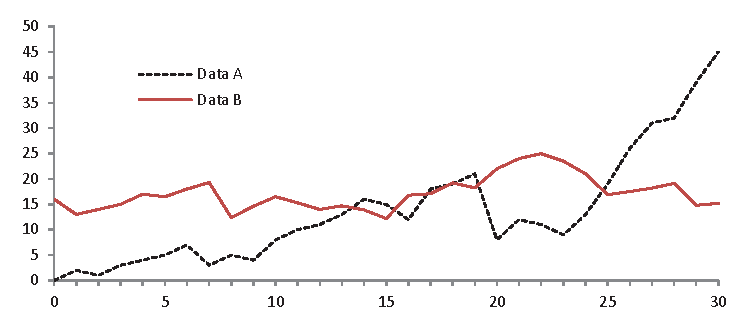
\includegraphics[width=\textwidth]{fig1.eps}
\caption{A figure caption is always placed below the illustration.
Please note that short captions are centered, while long ones are
justified by the macro package automatically.} \label{fig1}
\end{figure}

\section{ALTER TEXT, ev. noch nützliche Ideen/Formulierungen}
Our main attempt of modifying Alg.~\ref{alg:2} such that it incorporates the weaknesses of several neural networks is to hope for an improvement by incorporating the perturbations obtained for each network individually. In a first attempt, one could simply add up the perturbations stemming from two neural networks, see Alg.~\ref{alg:3}. As noted above, because of the norm-projection, this is different from our second attempt (given in Alg.~\ref{alg:4}), in which perturbations for the two networks are added up before projecting onto the norm constraint. Lines 14 and 15 in Alg.~\ref{alg:4} carry the main idea: 
{\bf After that, again the norm constraint is enforced Tun wir das wirklich???????}.
